\documentclass[11pt,twocolumn,oneside,openany,headings=optiontotoc,11pt,numbers=noenddot]{article}

\usepackage[a4paper]{geometry}
\usepackage[utf8]{inputenc}
\usepackage[T1]{fontenc}
\usepackage{lmodern}
\usepackage[ngerman]{babel}
\usepackage{ngerman}

\usepackage[onehalfspacing]{setspace}

\usepackage{fancyhdr}
\usepackage{fancybox}

\usepackage{rotating}
\usepackage{varwidth}

%Struktogramme
\usepackage[german,curves]{struktex}

\usepackage{pdflscape}
\usepackage{changepage}
\usepackage{graphicx}
\usepackage[bottom]{footmisc}
\usepackage{transparent}
\usepackage{graphbox}
\graphicspath{
	{Pics/PDFs/}
	{Pics/JPGs/}
	{Pics/PNGs/}
}
\usepackage{caption}
\usepackage{wrapfig}
\usepackage{marginnote}
\usepackage{tabularx}
\usepackage{dashrule}
\usepackage{soulutf8}
\usepackage{hhline}
%arydshln suppresses vertical lines in table
%\usepackage{arydshln}
\usepackage{multirow}
\usepackage{enumerate}
\usepackage[hidelinks]{hyperref}
\usepackage{listings}

\usepackage[table]{xcolor}
\usepackage{array}
\usepackage{enumitem,amssymb,amsmath}
\usepackage{interval}
\usepackage{cancel}
\usepackage{stmaryrd}
\usepackage{wasysym}
\usepackage{polynom}
\usepackage{diagbox}
\usepackage{dashrule}
\usepackage{framed}
\usepackage{mdframed}
\usepackage{karnaugh-map}
\usepackage{pdfpages}

\usepackage{blindtext}

\usepackage{eso-pic}

\usepackage{amssymb}
\usepackage{eurosym}

\usepackage[pages=some]{background}
\pagestyle{headings}
\renewcommand{\headrulewidth}{0.2pt}
\renewcommand{\footrulewidth}{0.2pt}
\newcommand*{\underdownarrow}[2]{\ensuremath{\underset{\overset{\Big\downarrow}{#2}}{#1}}}
\setlength{\fboxsep}{5pt}
\newcommand{\explainBelow}[3]{\underbrace{#1}_{\parbox{\widthof{#3}}{\footnotesize\raggedright #2}}}
\newcommand{\explainAbove}[3]{\overbrace{#1}^{\parbox{\widthof{#3}}{\footnotesize\raggedright #2}}}
\newcommand\footnoteref[1]{\protected@xdef\@thefnmark{\ref{#1}}\@footnotemark}


% Codestyle defined
\definecolor{codegreen}{rgb}{0,0.6,0}
\definecolor{codegray}{rgb}{0.5,0.5,0.5}
\definecolor{codepurple}{rgb}{0.58,0,0.82}
\definecolor{backcolour}{rgb}{0.95,0.95,0.92}
\definecolor{deepgreen}{rgb}{0,0.5,0}
\definecolor{darkblue}{rgb}{0,0,0.65}
\definecolor{mauve}{rgb}{0.40, 0.19,0.28}
\colorlet{exceptioncolour}{yellow!50!red}
\colorlet{commandcolour}{blue!60!black}
\colorlet{numpycolour}{blue!60!green}
\colorlet{specmethodcolour}{violet}

%Neue Spaltendefinition
\newcolumntype{L}[1]{>{\raggedright\let\newline\\\arraybackslash\hspace{0pt}}m{#1}}
\newcolumntype{M}{>{\centering\arraybackslash}X}
\newcommand{\cmnt}[1]{\ignorespaces}
%Textausrichtung ändern
\newcommand\tabrotate[1]{\rotatebox{90}{\raggedright#1\hspace{\tabcolsep}}}

%Intervall-Konfig
\intervalconfig {
	soft open fences
}

%Bash
\lstdefinestyle{BashInputStyle}{
	language=bash,
	basicstyle=\small\sffamily,
	backgroundcolor=\color{backcolour},
	columns=fullflexible,
	backgroundcolor=\color{backcolour},
	breaklines=true,
}
%Java
\lstdefinestyle{JavaInputStyle}{
	language=Java,
	backgroundcolor=\color{backcolour},
	aboveskip=1mm,
	belowskip=1mm,
	showstringspaces=false,
	columns=flexible,
	basicstyle={\footnotesize\ttfamily},
	numberstyle={\tiny},
	numbers=none,
	keywordstyle=\color{purple},,
	commentstyle=\color{deepgreen},
	stringstyle=\color{blue},
	emph={out},
	emphstyle=\color{darkblue},
	emph={[2]rand},
	emphstyle=[2]\color{specmethodcolour},
	breaklines=true,
	breakatwhitespace=true,
	tabsize=2,
}
%Python
\lstdefinestyle{PythonInputStyle}{
	language=Python,
	alsoletter={1234567890},
	aboveskip=1ex,
	basicstyle=\footnotesize,
	breaklines=true,
	breakatwhitespace= true,
	backgroundcolor=\color{backcolour},
	commentstyle=\color{red},
	otherkeywords={\ , \}, \{, \&,\|},
	emph={and,break,class,continue,def,yield,del,elif,else,%
		except,exec,finally,for,from,global,if,import,in,%
		lambda,not,or,pass,print,raise,return,try,while,assert},
	emphstyle=\color{exceptioncolour},
	emph={[2]True,False,None,min},
	emphstyle=[2]\color{specmethodcolour},
	emph={[3]object,type,isinstance,copy,deepcopy,zip,enumerate,reversed,list,len,dict,tuple,xrange,append,execfile,real,imag,reduce,str,repr},
	emphstyle=[3]\color{commandcolour},
	emph={[4]ode, fsolve, sqrt, exp, sin, cos, arccos, pi,  array, norm, solve, dot, arange, , isscalar, max, sum, flatten, shape, reshape, find, any, all, abs, plot, linspace, legend, quad, polyval,polyfit, hstack, concatenate,vstack,column_stack,empty,zeros,ones,rand,vander,grid,pcolor,eig,eigs,eigvals,svd,qr,tan,det,logspace,roll,mean,cumsum,cumprod,diff,vectorize,lstsq,cla,eye,xlabel,ylabel,squeeze},
	emphstyle=[4]\color{numpycolour},
	emph={[5]__init__,__add__,__mul__,__div__,__sub__,__call__,__getitem__,__setitem__,__eq__,__ne__,__nonzero__,__rmul__,__radd__,__repr__,__str__,__get__,__truediv__,__pow__,__name__,__future__,__all__},
	emphstyle=[5]\color{specmethodcolour},
	emph={[6]assert,range,yield},
	emphstyle=[6]\color{specmethodcolour}\bfseries,
	emph={[7]Exception,NameError,IndexError,SyntaxError,TypeError,ValueError,OverflowError,ZeroDivisionError,KeyboardInterrupt},
	emphstyle=[7]\color{specmethodcolour}\bfseries,
	emph={[8]taster,send,sendMail,capture,check,noMsg,go,move,switch,humTem,ventilate,buzz},
	emphstyle=[8]\color{blue},
	keywordstyle=\color{blue}\bfseries,
	rulecolor=\color{black!40},
	showstringspaces=false,
	stringstyle=\color{deepgreen}
}

\lstset{literate=%
	{Ö}{{\"O}}1
	{Ä}{{\"A}}1
	{Ü}{{\"U}}1
	{ß}{{\ss}}1
	{ü}{{\"u}}1
	{ä}{{\"a}}1
	{ö}{{\"o}}1
}

% Neue Klassenarbeits-Umgebung
\newenvironment{worksheet}[3]
% Begin-Bereich
{
	\newpage
	\sffamily
	\setcounter{page}{1}
	\ClearShipoutPicture
	\AddToShipoutPicture{
		\put(55,761){{
				\mbox{\parbox{385\unitlength}{\tiny \color{codegray}BBS I Mainz, #1 \newline #2
						\newline #3
					}
				}
			}
		}
		\put(455,761){{
				\mbox{\hspace{0.3cm}
\includegraphics[width=0.2\textwidth]{../../logo.pdf}}
			}
		}
	}
}
% End-Bereich
{
	\clearpage
	\ClearShipoutPicture
}

\setlength{\columnsep}{3em}
\setlength{\columnseprule}{0.5pt}

\geometry{left=2.50cm,right=2.50cm,top=3.00cm,bottom=1.00cm,includeheadfoot}
\pagenumbering{gobble}
\pagestyle{empty}

\begin{document}
	\begin{worksheet}{Berufliches Gymnasium}{Klassenstufe 13 - Mathematik}{Lernabschnitt 2: Grundbegriffe der Wahrscheinlichkeitsrechnung}
		\section{Zufallsexperiment}
		Ein Zufallsexperiment ist ein Prozess mit unbekanntem Ausgang, der sich beliebig oft unter gleichen Bedingungen wiederholen lässt\\
		\par\noindent
		\underline{\textbf{Beispiele:}}
		\begin{itemize}[label=-]
		\item Ein Würfel wird geworfen
		\item Passanten werden befragte, welche Partei sie zur Zeit wählen würden
		\item Sie nutzen die Straßenbahn-Linie 51 in Mainz ohne Fahrschein
		\end{itemize}
		\subsection{Merkmale eines Zufallsexperiments}
		Bei einem Zufallsexperiment lassen sich alle möglichen Ausgänge auflisten. Diese nennt man \underline{\texttt{Ergebnisse}} (mit der Abkürzung: \(e_1, e_2,\ldots\)).\\
		Nimmt man alle möglichen Ausgänge oder Ergebnisse zusammen, so nennt man diese Menge \underline{\texttt{Ergebnismenge}} (geschrieben mit: S = \({e_1, e_2, \ldots}\)).\\
		\par\noindent
		Betrachtet man jeden Ausgang einzeln, so kann jedem einzelnen eine Zahl zwischen 0 und 1 zugeordnet werden. Dieses gibt das Maß für die Möglichkeit des Auftretens an. Man bezeichnet dieses Maß auch als \underline{\textit{Wahrscheinlichkeit eines Ergebnisses/Ereignisses}} (Formal: \(P(e\ldots) = \ldots\)).\\
		Der Wahrscheinlichkeitswert von \grqq{}1\grqq{} heißt, dass das Ergebnis sicher eintritt. Beträgt die Wahrscheinlichkeit hingegen \grqq{}0\grqq{}, heißt das, dass das Ergebnis auf keinen Fall eintritt.\\
		Addiert man die Wahrscheinlichkeiten aller Ergebnisse, ergibt dies \grqq{}1\grqq{}.
		\subsubsection{Darstellung eines Zufallsexperiments als Baumdiagramm}
		\noindent
		\begin{wrapfigure}{L}{0.25\textwidth}
			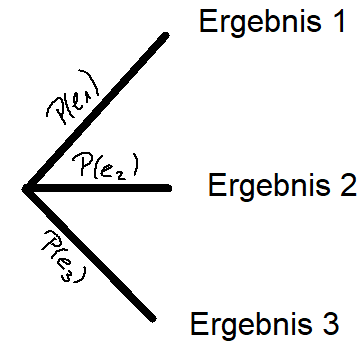
\includegraphics[width=0.23\textwidth,align=t]{../99_Bilder/04_WKR/baumEinf.png}
		\end{wrapfigure}
		\par\noindent
		Um ein Zufallsexperiment zu visualisieren gibt es diverse Möglichkeiten. Eines davon ist das Baumdiagramm. Dabei wird mit einem Ausgangsknoten begonnen, von welchem so viele Äste abgehen, wie es mögliche Ergebnisse gibt.
		\subsubsection{Tabellarische Darstellung der Ergebnisse mit den entsprechenden Wahrscheinlichkeiten}
		Es besteht auch die Möglichkeit, für ein Experiment mit einer endlichen Zahl an Ergebnissen eine Tabelle aufzustellen.\\
		\par\noindent
		\begin{tabularx}{0.48\textwidth}{|X|M|M|M|M|}
			\hline
			\shortstack{Ergebnis-\\se \(e_i\)} & \(e_1\) & \(e_2\) & \(\ldots\) & \(e_n\)\\
			\hline
			\(P(e_i)\) & & & & \\
			\hline
		\end{tabularx}
		\subsubsection{Darstellung als Diagramm am Beispiel \grqq{}Schwarzfahren in Berlin\grqq{}}
		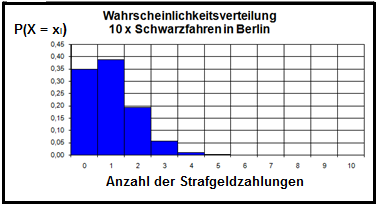
\includegraphics[width=0.48\textwidth]{../99_Bilder/04_WKR/darstEinf.png}\\
		\par\noindent
		Die Darstellung von Ergebnissen und ihren zugehörigen Wahrscheinlichkeiten nennt man auch \underline{Wahrscheinlichkeitsverteilung}.
		\subsection{Ereignis und Gegenereignis}
		Mehrere Ergebnisse kann man zu \textbf{\underline{Ereignissen}} zusammenfassen (geschrieben: \(A_1 = \lbrace{}e_1,\ldots\rbrace{}\)).\\
		\par\noindent
		\setlength{\leftskip}{0.5cm}
		\textit{Beispiel:} Beim Roulette-Spiel besteht das Ereignis \glqq{}gerade Zahl\grqq{} aus den Ergebnissen \(A_{gerade} = \lbrace{}2, 4, 6, \ldots\rbrace\).\\
		\par\noindent
		\setlength{\leftskip}{0cm}
		Als \underline{\textbf{Gegenereignis}} eines Ereignisses bezeichnet man alle Ereignisse, die nicht zum Ereignis gehören (Formal: \(\overline{A}\)).\\
		\par
		\setlength{\leftskip}{0.5cm}
		\par\noindent
		\textit{Beispiel:} Das Gegenereignis zu \glqq{}gerade Zahl\grqq{} beim Roulette ist \(\overline{A_{gerade}} = \lbrace{}0,1,3,\ldots,35\rbrace\).\\
		\par
		\setlength{\leftskip}{0cm}
		\par\noindent
		Häufig wird die Ergebnismenge zu \textbf{zwei} Ereignissen zusammengefasst (z.B. \(S = \lbrace\)Sie werden erwischt; Sie werden nicht erwischt\(\rbrace\); \(S = \lbrace\)SPD Wähler, kein SPD Wähler\(\rbrace\); \(S = \lbrace\)blond; nicht blond\(\rbrace\)).\\
		\par\noindent
		Auch zu Ereignissen gibt es Wahrscheinlichkeitsverteilungen.
		\subsection{Die Bestimmung der Wahrscheinlichkeit}
		Es gibt zwei Möglichkeiten für die Wahrscheinlichkeit eines Ergebnisses:
		\begin{itemize}
			\item \glqq{}Laplace\grqq{}-Wahrscheinlichkeit
			\item Empirische Wahrscheinlichkeit
		\end{itemize}
		\subsection{Laplace-Wahrscheinlichkeit}
		Sind alle Ergebnisse gleich wahrscheinlich, lässt sich die Wahrscheinlichkeit durch den folgenden Quotienten bestimmen:
		\[P(A_{\ldots}) = \frac{\text{Anzahl der Ergebnisse zum Ereignis}}{\text{Anzahl möglicher Ergebnisse}}\]
		\par\noindent
		\setlength{\leftskip}{0.5cm}
		\par\noindent
		\textit{Beispiel:} Wahrscheinlichkeit einen Bauer aus einem gut gemischten Kartenspiel zu ziehen:
		\[P(Bauer) = \frac{4}{32} = \frac{1}{8} = 0,125\]
		\par\noindent
		\setlength{\leftskip}{0cm}
		\subsection{Empirische Wahrscheinlichkeit}
		Will man z.B. die Wahrscheinlichkeit einer Zwillingsgeburt bestimmen, nutzt man Daten aus der Vergangenheit und bestimmt die relative Häufigkeit von Zwillingsgeburten.\\
		\par
		\setlength{\leftskip}{0.5cm}
		\par\noindent
		\textit{Beispiel:}\\
		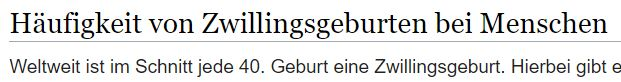
\includegraphics[width=0.48\textwidth]{../99_Bilder/04_WKR/zwillinge.jpg}\\
		\footnotesize{\texttt{Quelle: Wikipedia\footnote{https://de.wikipedia.org/wiki/Zwillinge}}}\\
		\normalsize
		\(\Rightarrow P(Zwilling) = 1:40 = 0,025\)\\
		\par
		\setlength{\leftskip}{0cm}
		\par\noindent
		Zur Ermittlung der Wahrscheinlichkeit wird das Zufallsexperiment häufig durchgeführt und die relative Häufigkeit wird bestimmt. Dabei \grqq{}pendelt\grqq{} sich die Wahrscheinlichkeit dann ein.
		\subsection{Mehrstufige Zufallsexperimente}
		Ein Zufallsexperiment kann sich auch aus mehreren einzelnen Experimenten zusammensetzen.\\
		\par
		\setlength{\leftskip}{0.5cm}
		\par\noindent
		\textit{Beispiel:} Zweimaliger Wurf einer Münze.\\
		Die Ergebnisse lassen sich nun entweder durch Zahlen oder Buchstabenpaare darstellen:
		\begin{align*}
			A_1 & = (K,\ K), & A_2 = (K,\ Z)\\
			A_3 & = (Z,\ K), & A_4 = (Z,\ Z)
		\end{align*}
		\par
		\setlength{\leftskip}{0cm}
		\par\noindent
		Häufig werden bei zweistufigen Experimenten die Ergebnisse nach der Anzahl des Auftretens eines bestimmten Ausgangs zu Ereignissen zusammengefasst.\\
		\par
		\setlength{\leftskip}{0.5cm}
		\par\noindent
		\textit{Beispiel:} Zwei Freunde spielen in einer ruhigen Mathestunde ein Spiel.\\
		\glqq{}Du gibst mit einen Euro und wirfst anschließend dreimal eine Münze!\grqq{}\\
		Pro geworfener \grq{}Zahl\grq{} gibt es 50 Cent zurück. Wird dreimal \grq{}Zahl\grq{} geworfen, gibt es 3 Euro zurück!\\
		\par\noindent
		Da für die Rückzahlung lediglich die \grq{}Zahl-Würfe\grq{} relevant sind, fasst man die möglichen Ergebnisse zu Ereignissen zusammen:
		\begin{itemize}[label=-]
			\item \(A_0 = {K,K,K}\)
			\item \(A_1 = {(Z,K,K),\ (K,Z,K),\ (K,K,Z)}\)
			\item \(A_2 = {(Z,Z,K),\ (Z,K,Z),\ (K,Z,Z)}\)
			\item \(A_3 = {Z,Z,Z}\)
		\end{itemize}
		\setlength{\leftskip}{0cm}
		\par\noindent
		\subsubsection{Darstellung als Baumdiagramm}
		Auch mehrstufige Zufallsexperimente lassen sich in einem Baumdiagramm darstellen. Dazu werden ausgehend vom Startpunkt so viele Äste gezeichnet, wie es Ergebnisse gibt. Von jedem möglichen eintretenden Ergebnis werden erneut so viele Äste wie mögliche Ergebnisse gezeichnet.\\
		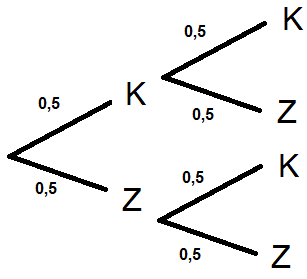
\includegraphics[width=0.48\textwidth]{../99_Bilder/04_WKR/zsBaum.png}\\
		\subsection{Wahrscheinlichkeiten  bei mehrstufigen Zufallsexperimenten}
		Für die Bestimmung von Wahrscheinlichkeiten bei mehrstufigen Zufallsexperimenten gibt es \textbf{zwei wichtige Regeln}. Diese simplen Regeln sollte man sich gut einprägen, da vieles Weitere auf Ihnen aufbaut.
		\begin{framed}
			\noindent
			\textbf{Pfadregel} (Wahrscheinlichkeit eines Ergebnisses)\\
			Multipliziere die \grqq{}Wahrscheinlichkeit entlang des Pfades, der dieses Ereignis beschreibt!\grqq{}\\
			\par\noindent
			\textbf{Additionsregel} (Wahrscheinlichkeit eines Ereignisses)\\
			Addiere die Wahrscheinlichkeiten aller Pfade, die zu einem Ereignis gehören!
		\end{framed}
	\end{worksheet}
\end{document}